\chapter{Caduta di Potenziale}
\begin{center}
    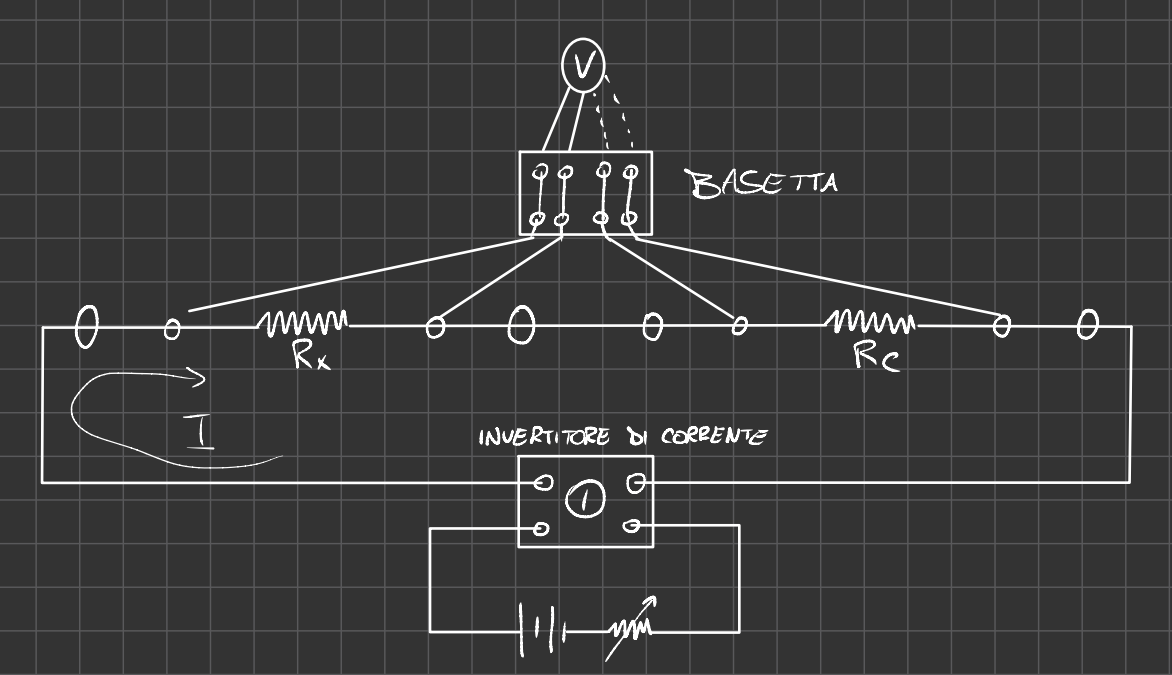
\includegraphics[width=.6\textwidth]{Images/figure43.png}
\end{center}
Questo metodo \textbf{voltamperometrico} viene usato per la misura di \textbf{resistenze di piccolo valore}, eliminando gli \textbf{effetti parassiti} delle \textbf{resistenze di contatto} e delle \textbf{forze elettromotrici di contatto}:
\section{Misurazione}
Vengono eseguite \textbf{quattro misurazioni in serie}:
\begin{itemize}
    \item $V_x$
    \item $V_c$
    \item Cambio verso alla corrente
    \item $-V_c$
    \item $-V_x$
\end{itemize}
\begin{equation*}
    \begin{dcases}
        V_x = R_x I\\
        V_c = R_c I
    \end{dcases}
    \implies V_x = R_x \frac{V_c}{R_c} \implies R_x = R_c \frac{V_x}{V_c}
\end{equation*}
\section{Incertezza}
Essendo:
\begin{equation*}
    V_x \approx V_c \implies \Delta x \approx \Delta c = \Delta
\end{equation*}
Quindi:
\begin{equation*}
    R_x = \frac{\hat{V}_x + \Delta}{\hat{V}_c +\Delta} R_c \implies R_x(\hat{V}_x , \hat{V}_c, \Delta, R_c) = f(...)
\end{equation*}
Calcoliamo l'\textbf{incertezza}:
\begin{equation*}
    \begin{aligned}
        u^2_{R_x} &= \left(\parti{f}{\hat{V}_x}\right)^2 \cdot u^2_{V_x} + \left(\parti{f}{\hat{V}_c}\right)^2 \cdot u^2_{V_c} + \left(\parti{f}{\Delta}\right)^2 \cdot u^2_{\Delta} + \left(\parti{f}{R_c}\right)^2 \cdot u^2_{R_c} =\\
        &=\left(\frac{\cancel{(\hat{V}_c + \Delta)R_c}}{(\hat{V}_c + \Delta)^{\cancel{2}}}\right)^2 \cdot u^2_{V_x} + \left(\frac{(\hat{V}_x - \Delta)R_c}{(\hat{V}_c + \Delta)^2}\right)^2 \cdot u^2_{V_c} + \\
        &+\left(\frac{(\hat{V}_c - \hat{V}_x) R_C}{(\hat{V}_c + \Delta)^2}\right)^2 \cdot u^2_{\Delta} + \left(\frac{\hat{V}_x + \Delta}{\hat{V}_c + \Delta}\right)^2 \cdot u^2_{R_c} =\\
    \end{aligned}
\end{equation*}
Considerando $\Delta \approx 0$ possiamo scrivere:
\begin{equation*}
    = \frac{R^2_c}{\hat{V}^2_c} \cdot u^2_{V_x} + \frac{R^2_c \hat{V}^2_x}{\hat{V}^4_c} \cdot u^2_{V_c} + \frac{\hat{V}^2_x}{\hat{V}^2_c} \cdot u^2_{R_c}
\end{equation*}
Calcoliamo quindi l'\textbf{incertezza} \textbf{relativa} come:
\begin{equation*}
    \dot{u}_{R_x} = \frac{u_{R_x}}{R_x} = \sqrt{\frac{u^2_{V_x}}{\hat{V}^2_x} + \frac{u^2_{V_c}}{\hat{V}^2_c} + \frac{u^2_{R_c}}{R^2_c}}
\end{equation*}
Notiamo quindi che \textbf{più le tensioni sono elevate e meno incertezza su $R_x$ avremo}.
\section{Resistore a 4 morsetti}
In questo tipo di sistema, abbiamo utilizzato resistori a 4 morsetti, dove:
\begin{center}
    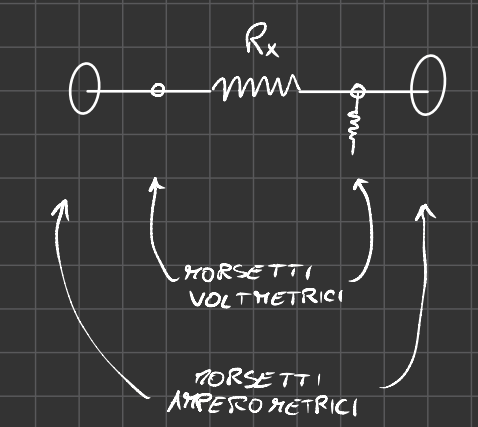
\includegraphics[width=.2\textwidth]{Images/figure44.png}
\end{center}
\begin{itemize}
    \item I due esterni sono detti morsetti amperometrici
    \item I due interni sono detti morsetti voltmetrici
\end{itemize}

